\documentclass[11pt]{article}


\usepackage{fullpage}
\usepackage{graphicx}
\usepackage{amsmath}
\usepackage{amssymb}
\usepackage{amsthm}
\usepackage{fancyvrb}

\newcommand{\myname}{Mehshan Mustafa}

\newenvironment{theorem}[2][Theorem]{\begin{trivlist}
\item[\hskip \labelsep {\bfseries #1}\hskip \labelsep {\bfseries #2.}]}{\end{trivlist}}
\newenvironment{lemma}[2][Lemma]{\begin{trivlist}
\item[\hskip \labelsep {\bfseries #1}\hskip \labelsep {\bfseries #2.}]}{\end{trivlist}}
\newenvironment{exercise}[2][Exercise]{\begin{trivlist}
\item[\hskip \labelsep {\bfseries #1}\hskip \labelsep {\bfseries #2.}]}{\end{trivlist}}
\newenvironment{problem}[2][Problem]{\begin{trivlist}
\item[\hskip \labelsep {\bfseries #1}\hskip \labelsep {\bfseries #2.}]}{\end{trivlist}}
\newenvironment{question}[2][Question]{\begin{trivlist}
\item[\hskip \labelsep {\bfseries #1}\hskip \labelsep {\bfseries #2.}]}{\end{trivlist}}
\newenvironment{corollary}[2][Corollary]{\begin{trivlist}
\item[\hskip \labelsep {\bfseries #1}\hskip \labelsep {\bfseries #2.}]}{\end{trivlist}}
\newenvironment{solution}{\begin{proof}[Solution]}{\end{proof}}
\newenvironment{idea}[2][Proof Idea.]{\textit{#1} #2}



\parindent0in
\pagestyle{plain}
\thispagestyle{plain}

\usepackage{csquotes}
\usepackage[shortlabels]{enumitem}

\newcommand{\dated}{\today}
\newcommand{\token}[1]{\langle \text{#1} \rangle}

\begin{document}

\textbf{Introduction to the Theory of
Computation}\hfill\textbf{\myname}\\[0.01in]
\textbf{Chapter 5: Reducibility}\hfill\textbf{\dated}\\
\smallskip\hrule\bigskip

\begin{problem}{5.20}
Prove that there exists an undecidable subset of $\{1\}^{*}$.
\end{problem}

\begin{idea}[Proof Idea.] Let $\mathcal{L} = \mathcal{P}(\{1\}^{*})$ be the set of all subsets of $\{1\}^{*}$. To show that there exists an undecidable member of $\mathcal{L}$, we first observe that the set $\mathcal{B}$ of all \textit{infinite binary sequences} is uncountable. We show that $\mathcal{L}$ is also uncountable by giving a correspondence with $\mathcal{B}$.
If $\mathcal{L}$ is uncountable, then it would imply that there exists an undecidable member of $\mathcal{L}$, because $\mathcal{L}$ is a bigger set than the set of all Turing machines, which we know is countable according to the Corollary 4.18.
\end{idea}

\begin{proof}
The proof is based on the proof of Corollary 4.18. An infinite binary sequence is an unending sequence of 0s and 1s. Let $\mathcal{B}$ be the set of all infinite binary sequences. We show that $\mathcal{B}$ is uncountable by using diagonalization. Suppose that the correspondence $f$ exists between $\mathcal{N}$ and $\mathcal{B}$ as shown in the table below. We construct the desired $x$ by giving its infinite binary sequence. Our objective is to ensure that $x \neq f(n)$ for any $n$. To ensure that $x \neq f(1)$, we let the first character of $x$ to be different from the first character of $f(1)=\underline{1}000101\cdots$, which is 0. To ensure that $x \neq f(2)$, we let the second character of $x$ to be different from the second character of $f(2)=1\underline{0}01101\cdots$, so we choose 1. Continuing in this way down the diagonal of the table for $f$, we obtain all the characters of $x$, as shown in the following table. We know that $x$ is not $f(n)$ for any $n$ because it differs from $f(n)$ in the $n$th character.

\begin{center}
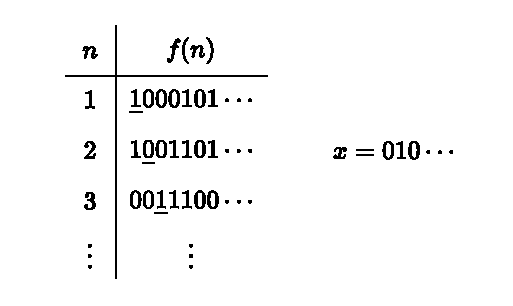
\includegraphics[scale=0.8]{Figures/Problem5.20a.pdf}
\end{center}

We show that $\mathcal{L}$ is uncountable by giving a correspondence with $\mathcal{B}$, thus showing that the two sets are the same size. Let $\{1^{*}\} = \{s_1, s_2, s_3, \cdots\}$. Each language $A \in \mathcal{L}$ has a unique sequence in $\mathcal{B}$. The $i$th bit of that sequence is a 1 if $s_i \in A$ and is a 0 if $s_i \notin A$, which is called the characteristic sequence $\mathcal{X}_A$ of $A$.

\begin{center}
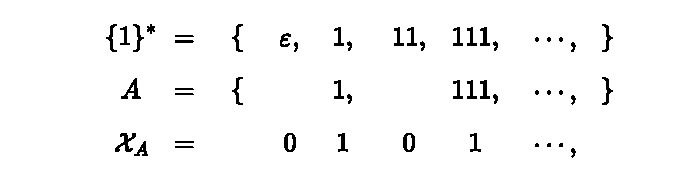
\includegraphics[scale=0.8]{Figures/Problem5.20b.pdf}
\end{center}

The function $f:\mathcal{L}\longrightarrow\mathcal{B}$, where $f(A)$ equals the characteristic sequence of $A$, is one-to-one and onto, and hence is a correspondence. Therefore, as $\mathcal{B}$ is uncountable, $\mathcal{L}$ is uncountable as well.
\end{proof}
\end{document}